\documentclass[a4paper,superscriptaddress,nofootinbib]{revtex4}

\addtolength{\oddsidemargin}{1cm}
\addtolength{\evensidemargin}{1cm}
\addtolength{\textwidth}{-2.6cm}

% Packages
\usepackage[caption=false]{subfig}  % needed for compatibility btw revtex and captions
\usepackage{dcolumn}   % needed for some tables
\usepackage{graphicx}
%\usepackage{titlesec}
\usepackage{amsmath}
\usepackage{amssymb}
\usepackage{amsthm}
  \newtheorem{theorem}{Theorem}
  \newtheorem{lemma}[theorem]{Lemma}
  \newtheorem{definition}[theorem]{Definition}
\usepackage{tikz}
\usepackage[utf8]{inputenc} % for at få danske karakterer. Kræver at alle bruger en editor som understøtter utf8.

% Macros
\definecolor{mygreen}{rgb}{0,0.6,0}
\newcommand{\at}{\makeatletter @\makeatother}
\newcommand{\tmin}{t_{\min}}
\newcommand{\tmax}{t_{\max}}

\iffalse
% Style parameters
\setlength{\parskip}{0pt}
\setlength{\tabcolsep}{6pt}
\setlength{\arraycolsep}{2pt}
\titlespacing*{\section}
{0pt}{2ex}{1ex}
\titlespacing*{\subsection}
{0pt}{2ex}{1ex}
\titlespacing*{\subsubsection}
{0pt}{2ex}{1ex}
\fi

\graphicspath{{../plots/}{../images/}}


\usepackage{zref-xr,zref-user}
\zexternaldocument*{"PLOS ONE/cd"}

\begin{document}

\title{Supplementary Material for \\
The Curse of Shared Knowledge: Recursive Belief Reasoning in a Coordination Game with Imperfect Information}
\author{Thomas Bolander}
%\affiliation{Department of Applied Mathematics and Computer Science, Technical University of Denmark, Richard Petersens Plads, building 324, DK-2800 Lyngby, Denmark}
\author{Robin Engelhardt}
\author{Thomas S. Nicolet}
%\affiliation{Center for Information and Bubble Studies, Department of Communication, University of Copenhagen, Karen Blixens Plads 8, DK-2300 Copenhagen S.}

\maketitle
%\normalsize
%\onecolumngrid

% NB: Requires formatting

\iffalse
\section*{This PDF includes:}
Supplementary text \\
Figs FIG.1 to FIG.7 \\
Table 1\\
Captions for Databases \\
References for SI citations 


\clearpage
%\appendix
\fi

%{\Huge \center Supplementary Information\\}


\section{Materials and Methods}

\subsection{Mechanical Turk (MTurk) Experiment, Including Walkthrough and Screenshots}
\begin{figure} %[h]
\centering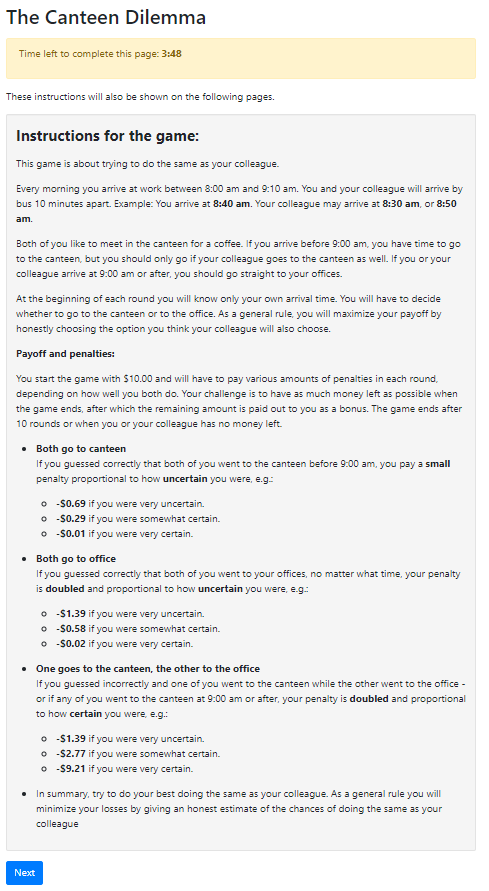
\includegraphics[width=0.8\linewidth]{screenshot_instructions}
\caption{Screenshot of instructions page.}
\label{fig:instructions}
\end{figure}
\begin{figure} %[h]
\centering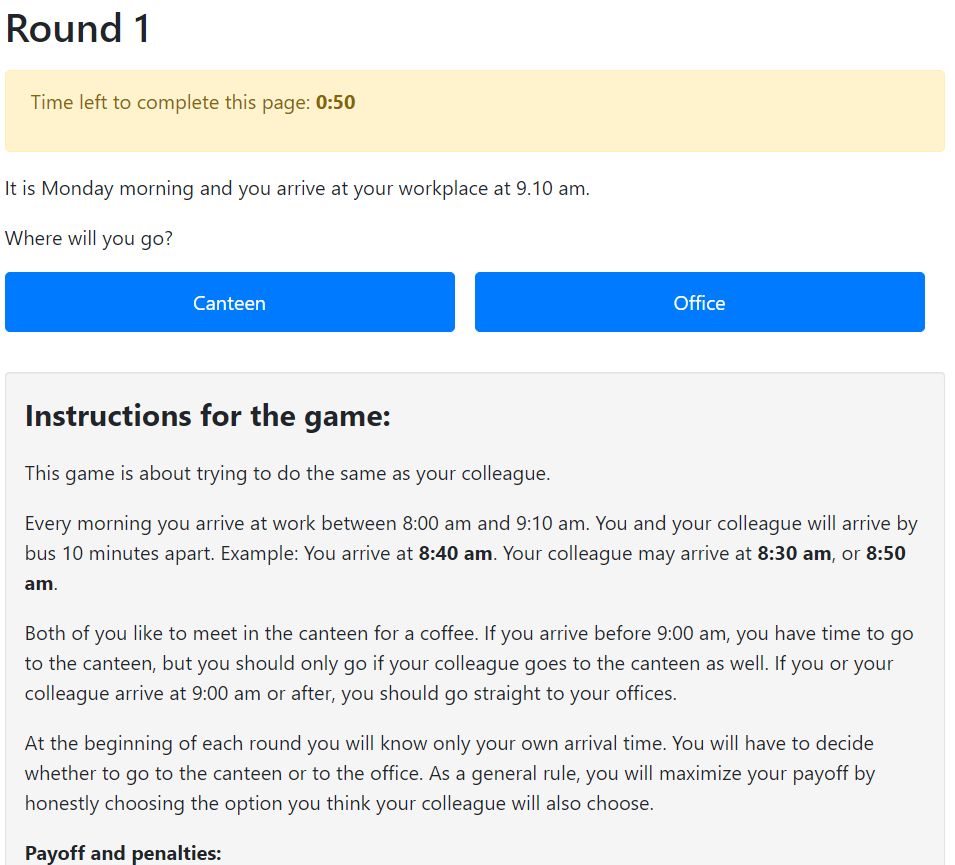
\includegraphics[width=0.8\linewidth]{screenshot_round1}
\caption{Screenshot of choice page, round 1.}
\label{fig:round1}
\end{figure}
\begin{figure} %[h]
\centering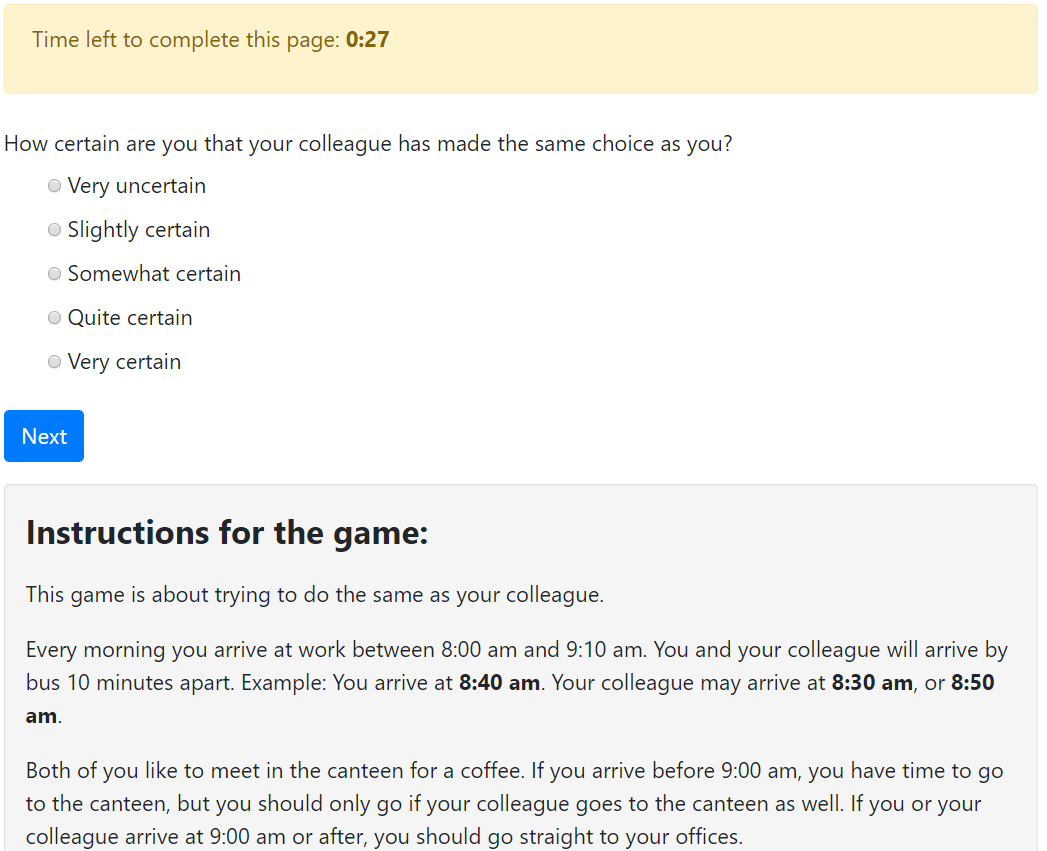
\includegraphics[width=0.8\linewidth]{screenshot_certainty}
\caption{Screenshot of page where participants had to estimate the probability that their colleague would make the same choice.}
\label{fig:certainty}
\end{figure}
\begin{figure} %[h]
\centering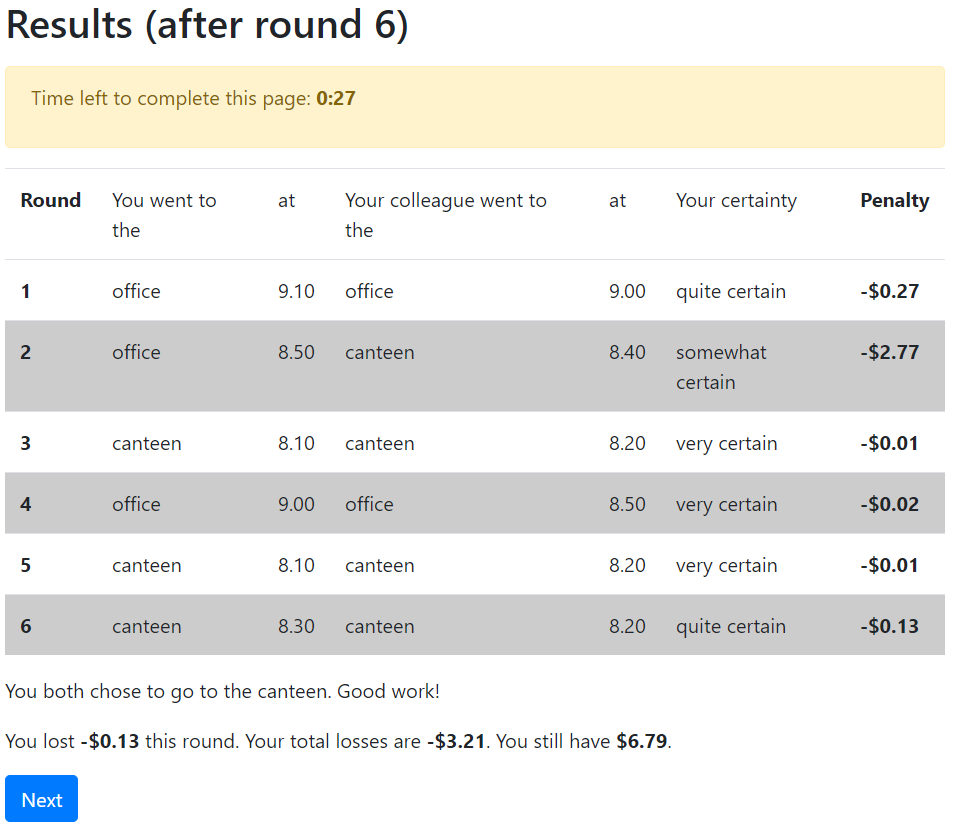
\includegraphics[width=0.7\linewidth]{screenshot_round6results}
\caption{Screenshot of results page, round 6.}
\label{fig:results6}
\end{figure}
\begin{figure} %[h]
\centering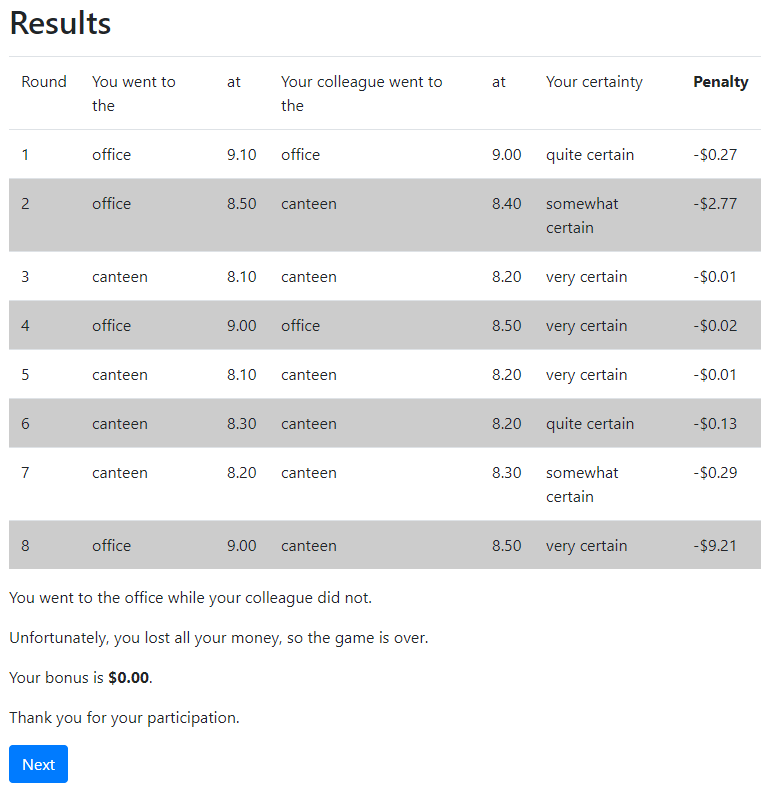
\includegraphics[width=0.7\linewidth]{screenshot_round8finished}
\caption{Screenshot after a player has lost all her bonus.}
\label{fig:round8finished}
\end{figure}
The MTurk experiments were approved by the the Research Ethics Committee at the Faculty of Humanities, University of
Copenhagen, Denmark on 22 February 2019. The approval stated: 
\begin{quote} 
The Research Ethics Committee at the Faculty of Humanities, University of
Copenhagen, has assessed your research experiment “The Canteen Dilemma“. Based
on the information you have provided in your Application for Ethical Approval, the
Committee has concurred that the project activities are in accordance with the relevant
International and Danish ethical guidelines and regulations. [...] The Committee hereby approves your project.
\end{quote} 
MTurk participants were recruited, and online experiments were conducted in the period from the 25th February 2019 to 1st March 2019. After accepting
%After accepting  
our `Human Intelligence Task' (HIT) and providing informed consent, participants from MTurk were put in a ’waiting room’ until they were paired up with another participant. After a group of two was formed, participants were directed to an initial instruction page which detailed the rules of the game with a time limit of 240 seconds, see screenshot in Fig.~\ref{fig:instructions}.
After reading the instructions, participants were directed to round 1 (of 10) where they were given their own arrival time and asked to make a decision between between going to the canteen or the office. Each round had a time limit of 61 seconds and rules from the instructions were repeated on the bottom of the page, see example screenshots for round 1 in Fig.~\ref{fig:round1}.

After making their decision (`Canteen' or `Office'), participants were asked to estimate how certain they were that the other player made the same choice as them, ranging from `very uncertain' over `slightly certain', `somewhat certain' and `quite certain' to `very certain', see Fig.~\ref{fig:certainty}.

After both players have made their choices and their certainty estimates, they are prompted to a results page showing them the results of the previous rounds, including arrival times for both players, their choices, their own certainty estimate and resulting payoff, see example screenshot after round 6 in Fig.~\ref{fig:results6}. After 30 seconds, the game would automatically proceed to the next round.

In many instances, groups were not able to play the maximal number of rounds, because one or both of the participants had lost all their bonuses. An example of such a situation is shown in Fig.~\ref{fig:round8finished}. In such cases, the game would end for both players and they were asked to answer a follow-up question: 


\begin{quote}
\indent
1. ``The game is over. Do you think it was your fault it is over, your colleagues fault, or do
you think it was because of some other reason?'' \textit{(Possible answers: `My fault', `Other's fault', `Other reason')}
\end{quote}
This question probes into participants' ability to rise above their possibly myopic understanding of the game. In addition to this question, all participants were asked three additional post-game questions about their strategy of play and their understanding of the game. The first was:
\begin{quote}
\indent
2. ``What strategy did you use while playing this game?" \textit{(open ended)}
\end{quote}
The answers to this question provided insight into the reasoning and thoughts of the participants. The next question was used to gauge the depths of recursive reasoning and reads:
\begin{quote}
\indent
3. ``Imagine you could have agreed beforehand with your colleague about a point in time where it is safe to go to the canteen. What time would that be?" \textit{(`I don't know', `There is no such time', 8:00, 8:10, 8:20, 8:30, 8:40, 8:50, 9:00, 9:10)}
\end{quote}
A final question pertaining all participant's understanding of the concept of common knowledge was the following:
\begin{quote}
\indent
4. ``Imagine you arrive at 8:10 am. Is it common knowledge between you and your colleague that it is safe to go to the canteen, that is, you both arrived before 9:00 am?''. \textit{(`Yes', `No', `Don't know')}
\end{quote}


\subsection{DTU Experiments}
The DTU students were asked three additional post-game questions:
\begin{quote}
5. ``Did you ever go to the canteen at an arrival time later than what was safe according
to your previous answer? Why or why not?'' \textit{(open ended)}
\end{quote}
\begin{quote}
6. `Did you ever choose differently after seeing the same arrival time again at a later point
in the game? Why or why not?" \textit{(open ended)}
\end{quote}
\begin{quote}
7. `Imagine you arrived at [8:40/9:00] and you have been secretly informed that your colleague’s arrival time is 8:50. Where do you think your colleague will go?'' \textit{(`Canteen', `Office')}
\end{quote}
In the last question, half of the participants were given 8:40 as their own arrival time while the other half were given 9:00. The question concerns whether player’s own knowledge of the other’s arrival time affect their prediction of the other player’s decision. It relates to the curse of knowledge \cite{birch2007curse} since participants might attribute their own belief (that it is early enough or too late to go to the canteen) to the other player.

\subsection{MTurk Settings}
\label{MTurksettings}
Looking at Table \ref{table:A1}, the average payout to MTurk-workers was \$4.17 (including a general participation fee of \$2) which amounts to an average of more than \$20 per hour, which is considered very generous according to MTurk guidelines and certainly above the recently estimated average of \$6 per hour when excluding un-submitted and rejected work \cite{HaraEtAl18}. Students in the DTU experiments (DTU1 and DTU2) did not receive any monetary reward, but were told to try to maximize their payoff, and awarded prizes for doing well.

\begin{table} %[h]
\centering
\begin{tabular}{lccccc}
\hline
Experiment   &   Participants &   Attrition rate &   N & Rounds & AvgPayout  (\$) \\
\hline
 MTurk 	& 714 &  0.02 &  680 & 10 & 4.36    \\
 DTU1  	& 106 &  0.13 &  80 & 30 & (prizes)   \\
 DTU2  	&   50 &  0.08 &  42 & 30 & - \\
\hline
\end{tabular}
\caption{The main experiment on Amazon Mechanical Turk (MTurk) had 714 participants of which 17 participants (2,4 \%) quit prematurely, some of them quite early in the game. These quitters were told (in the consent form) that they would receive no bonus and no participantion fee. They are excluded from the data analysis. Their ``lucky'' colleagues however, got both their bonuses and participation fee, but are likewise excluded from the data analysis. Therefore the final number of subjects, $N$, is reduced by twice the attrition rate. In the two DTU experiments with students from the Technical University of Denmark (DTU1 and DTU2) attrition rates were slightly higher, mainly due to the higher number of rounds played.}
\label{table:A1}
\end{table}

Participants quitting a study before completing it is prevalent on MTurk, and varies systemically across experimental conditions \cite{ZhouFishbach16}. In our experiments on Amazon Mechanical Turk attrition rates were $2\%$, witnessing that we had managed to design the experiment in a way that minimized drop-out rates. A combination of high payouts, a logarithmic scoring rule taking advantage of loss aversion biases, a consent form stipulating the revocation of the participation fee after dropout, and minimization of waiting times may have been the main reasons.

All participants automatically received a `qualification' when accepting a HIT. This qualification ensured that participants could not play the game again. In addition, we required that participants should have had completed at least 500 HITs, have an accepted HIT rate of 98\% or above, and should be from the United States or Canada. This ensured that we would get relatively experienced and qualified participants.

MTurk participant attention was expected to be equal to or better than undergraduate participant's attention \cite{Rand2012}, while various forms of dishonesty (practical joking or trying to pair up with a friend) was expected to be rare, due to the high turnover rate experienced for our HITs. In addition, during the experiment, participants had easy access to our email for questions and possible bug reports. Apart from a few timeouts, participants had no comments or complaints.

\subsection{Full Rule Set for DIS Version of the Game}

This game is a 2-player cooperative coordination game with 15 rounds. The 2 players have to try to coordinate their actions, and if they are successful, they will both achieve the same positive reward (so it's not a zero-sum game). The positive reward can either be \$1 or \$2. If you're miscoordinated, you lose all the money you earned so far in the game. After the 15 rounds, you get to keep the rewards you have accumulated. Well, actually, in this version of the game, you will not be paid actual money, but you should try to behave as if you did, i.e., try to maximize the reward.

  

In each round, each player is dealt a face down card. On the face of the card there is a number in the interval 2--10 (it's a card from a deck of standard playing cards). The numbers on the two dealt cards are always exactly 1 apart, so if for instance one of the players gets a 3, then the other will either be getting a 2 or a 4. And since 10 is the maximum, if one player gets a 10, necessarily the other player is getting a 9. And similarly, if one gets a 2, necessarily the other gets a 3.  

When the cards are dealt, each player looks at the number on their own card without showing it to the other. The two players are not allowed to communicate or exchange any kind of information during the game. After each player has inspected their own card, they should hide either a white or a black marble stone in their hand and put the hand on the table. Each player has to make an individual choice without communicating with or revealing it to the other player. 

When both players have their closed hands with the hidden stones on the table, they wait for the facilitator to tell them that now they can open their hands to reveal the two stones, and they can also turn their cards to reveal their numbers.  

Both players then receive rewards depending on the colors of their stones and the numbers on their cards. The white marble stone is worth \$2, and the black marble stone is worth \$1, but you only get to keep your stones (money) if you choose the same stone as the opponent, and additionally, if you both choose the white stones, you only get to keep them if both card numbers are strictly below 9. In more details:  
\begin{enumerate}
\item[a)] If one player chose a white stone and the other a black stone, then they both lose all the stones (money) they have received in the game so far.
\item[b)] If both players chose a black stone, they both receive \$1 (i.e., a black stone).
\item[c)] If both players chose a white stone, then they both receive \$2 (i.e., a white stone), but only if both numbers are strictly below 9, meaning they are both in the interval 2--8. If not, the players lose all the money (stones) they have received in the game so far.
\end{enumerate} 

\section{Results} 

\subsection{Transcriptions of Qualitative Interviews with DIS Students}


\paragraph{Interview 1}
This is a transcription of an interview between Robin Engelhardt (R) and students (S) from the DIS experiment.


\medskip
R: .. Okay. I'll ask you some questions, and then maybe if I don't pin anybody of you out, just the first one who would like to answer answers. Okay, so the first question would be 
“Did you believe that your co players received the same rules as you yourself?” 

S: “Yes.“

R: “Right. That should be quite obvious. And that was the problem with the games online, because some people think, oh, yeah, but we can invent new rules for each player. They cannot know that the others know. Okay, next question:

R: “Were you uncertain about the rules and whether your co-payer had understood the rules?” 

S: “Yes.”

R: “Okay. How may we start with you? In what sense were you uncertain?” 

S: “I don't know. It took me reading it over a few times, I guess.” 

R: “Okay, and then you thought your coplayer might as well have some problems understanding it?”

S: “Yeah, kind of about being on the same page.“

R: “And when did you think you were okay, you both knew how the rules were? At what point? In which round?”

S: “One round. Because we both, like, played it and then realized this is why we did it.” 

R: “What about you? You said also yes.” No?”

R: “Okay. So, what about you? Did you think I didn't understand the rules? So did you think you were completely clear about the rules?” 

S: “I think we both understood it.” 

R: “Okay.” 

S: “You know, I wasn't uncertain.”

R: “You weren’t uncertain at all? Okay. That's the benefits of being in the same room, I guess. So, do you think it was your fault, the game, you miscoordinated? Or was it your partner's fault? Or do you think it was because of some other reason? So now anybody of you we miscoordinated once, we all miscoordinated at one point. Right. Whose fault was it? Whose error?”

S: “I don’t think it was anybody’s fault. It was the strategy?” 

S: “I don't think she ever made a decision that I would think was objectively a wrong decision.” 

R: “And you never thought that. You thought that about me at one point when I chose the black stone instead of the white one. You had a seven, I had a six. I could have had an eight. Okay, so now the more substantial. Yeah, but I would like to hear …”

S: “because we are trying to remember what happened, we're trying to figure out the scenario. One sort of scenario is neither of our faults. “

S: “We kind of end up developing the strategy that because we had so much so late in the game, might as well play it safe. “

R: “So, what was safe?”

S: “Black.“

S: “Yeah, black is safe, always. Right. Any combo. If both people have black.” 

R: “Yes. You didn't do that. Okay. Would you have done that? “

S: “You'd have to be able to communicate with your partner. Which technically we weren't supposed to do. “

R: “Yes, exactly.”

S: “Otherwise, you'd lose out on a lot before your partner figured out you were trying to do it. “

S: “If I was playing with somebody who I knew better and had played games with before and knew if they played more riskier, more safe, I think it would have been easier to know what we're doing without being okay. “

R: “When did you find out that the black was a safe strategy? “

S: “I think we always did. But I think the big thing, as we started to get more and more altogether, we didn't want to lose them all. So, then I think that's when it hit me that I was like, oh, I just play black.”

S: “In round eight, or something like that?”

S: “Yeah. Okay. I know we're in the same room as a bunch of other people playing it, but I would see that we had more than everyone else and I kind of wanted to stay on top of everyone else. “
S: “Okay, so it's due to the comparison of the others you found out maybe safe way is to always choose black even though it is a lower payoff.”

R: “Did you other guys think about that?” 

S: I thought that black is dangerous because if one person plays black, you lose everything because the other one probably chooses white.”

R: “So, what was your strategy then? 

S: “Also, to play most conservatively, but there's like near like the 7-8-9-7-8 range that's like then I usually play up for black. Below that I play for white.” 

R: “Okay, so let me understand. If you have an eight, you take black?”

S: “..and I also think like two spots in either direction compensate for what the partner would think. “

R: “Okay, so seven, you would choose black as well? “

S: “Yeah, I think so.”

R: “Six, you would choose white? At least that you did, I remember. “

S: “Seven you would have to think about they might have an eight and then…

S: “ But if they have a six…Right. If you play the seven, assuming that yeah,..”

S: “…it was kind of weird because I was thinking because with eight, statistically speaking, it makes more sense to pick black because if they have a nine, they're always going to pick black. If they have a seven, they might anticipate you, they might not. Technically, there's a chance that they choose black still. So if you look at it from peer statistics, it makes more sense to pick black eight, but by the same token, as a seven, it makes more sense to pick white because the 6 is basically always going to pick white, and on the 8th they might pick white, they might not.”

R: “Yeah…. Did you have an idea of what a safe strategy would be? What strategy did you use?”

S: “I don't know. I've decided, as I saw the plan, lower than a certain number, I would only use white. If it was like a higher number, I would think about it.”

R: “What was the cut-off number?”

S: “Seven.”

R: “So seven would be white?”

S: “I don't know.“

R: “Okay, I'll find out. Okay. So, it seems that most of you chose some kind of probability measure about what to choose when having a seven or eight. Is that true? Or did you think, okay, black is always safe, so why not black, for instance? “

S: “I don't think the money or is enough for me to want to care. The black was a million dollars and the white was like 2 million, like double. I would always choose black because I'm happy with a million dollars, but if it's one and $2, I don't care about one and $2. “

R: “Okay…”

S: “ so I'd rather have more than like ..:”

R: “But if you would have chosen black all the time from the beginning, if it were a million dollars, you might have a guy choosing white and you'll just bust. “

S: “Yeah, I know, but I'm saying I feel like if the money was more, I want to play, like, a safer strategy, but since the money is negligible, I don't care about selling the safe strategy. “ % TSN: The absolute win/losses may be relevant for the game theory, i.e. in a game where you cannot afford to lose (even just due to opportunity cost), the game may change

R: “Yeah, but my question is what is safe? What is the most safe strategy? Right. Even though you might know that black, if both could agree on always choosing black, it would be fine, but it's not sure. There still wouldn't be the most safe strategy, right? Because you don't know. Maybe the guy chooses white once in a while when he gets a two or three.”

S: “I feel like maybe if it's like 15 rounds, if I played like the first all ten rounds, all black, then he would get the hit and at least you'll get 5 million in the end and I'd be pretty happy walking away.”

S: “There's also the cut off ones where if you had a two or three, you would obviously play.  There'd be no sense in playing black. There's not even a chance that they have one that white wouldn't work out. If you had a two, then you know the other person is a three or three. You know they have two or four. At that point you would play white because you would do more because that's safe no matter what.”

S: “The safest is always play white, like two to five there's no risk involved in the numbers…. “ % TSN: Relevant in article

R: “There's absolutely no risk involved. … from five low or from where?”

S: “From five and lower.”

S: “Well, that's where I was thinking about that a couple of times because it gets a little weird in that. Like…”

R: “Do you personally have five and lower?”

S: “Except since you're saying there's risk involved in six, there's technically also risk involved in five. “

S: “Okay, if they have a seven, they might think you have an eight. That's where the risk comes. It doesn't go lower than that. If you have a six, you could be mistaken for having an eight, and that's where the risk comes from. If you have a five, you're not going to be mistaken for having any …”

S: “Yeah, but the point, too, is you could decide with that six that since you might be mistaken for having an eight, that you should go black.”

S: “Two to five is white, six to ten is black, except and then you always win.”

S: “No, because if you have a six and a five and you use that paradigm, you lose. “

S: “No, but it's if you personally have a five if I personally have a five, then I know that they either have a six or five. So even if I know the max, they can have six. Even when they're a six, they're still going…”

S: “ to but if the six then goes, okay, it makes sense for me to go black because they could think that I could have eight. “

S: “Then it doesn't work”

S: “No, the cut off is weird. I was thinking about that earlier. I didn't go super in depth, but I was like, yeah, if you dig into this deep enough, it could like, cascade and be like, well, at this cut off, they could think ..

S: “Ok, this it's not 100\% like they …”

R: “You used cut off at seven, right? We did both more or less right, though I failed once. Do you think? Now we are talking about cut off. It's very interesting because you were, at least in the start, sure that it would be completely safe with five below to take white. If you could have talked beforehand before the game started, what is our cut off? And you could have decided it is five, would you then always win?” 

S: “No, it's always possible.” 

S: “Having one number be 50 50. “

R: “Yeah, maybe that's a good idea. What about if you had a three? Do you think it is common knowledge that both of you are below eight?”

S: “Yes”

R: “..and common knowledge in the sense of common knowledge, in the sense of logic or in the sense only of common sense? “

S: “I think it's logic, because if you have a three, the max they have is four. So, the max they could think you have five, which is six. “

R: “So, you're studying logic. What is it called? AI. What is it? AI. So, you have a lot of logic with Thomas, so you understand the concept of coming out. You have heard about it. Everybody knows that. Everybody knows broadcasting messages. So, we expect everybody to know that. “

R: “Did you did you ever choose differently after seeing the same number again at a later point in time? So, imagine you chose seven. You chose white, getting a seven, which was white, and then later you get a seven and you chose black, something like that. So, getting the same number, choosing differently later, did we do that? “

S: “Yeah, I did that with you. After we lost, all of ours were low again. We were playing it safer and wanting to get more money when it was safe”.

R: “So, you played it safe. More black choices when you had a lot of money?”

S: “Yeah, because we didn't want to lose everything we got.”
 
R: “You did that?”

S: “The more money we got, the things that we got, and then when we lost it, we reset to just like ..”

R: “Okay, imagine you get a number, say, seven, and you have been secretly informed that your colleague's number is eight. What do you think?

S: “That happened to me…. she was thinking, and I had a seven, so I'm like, if she had a six, she wouldn't have been thinking. Yes…” 

R: “And so you read her, cold reading?”

S: “Hm..mm”


R: “Okay. And you said she has an eight, and she is contemplating black.“

S: “Yes.”

R: “And what happened?”

S: “I played a white. She played a black. Like, you would actually know what decision she will make. “

R: “Yes. Did you learn that choosing white with the number eight was dangerous? Yes? I guess everybody likes that. If yes, why was choosing white with the number seven not dangerous?”

S: “It was.”

R: “It was less dangerous?”

S: “Yeah, it's less dangerous because with eight, there is a 50\% chance that they're guaranteed to choose black with the seven there's a 50\% chance that they're almost guaranteed to choose white, because most of the time…white.”

S: “But logically, if they choose black with eight, it's also not very safe to choose white with seven. Right? “

S: “Yup. Seven, if you chose white, you know that your partner should choose white and could choose white. But the only thing you were going against, like, your partner. “

S: “Yeah. Your partner might think you have nine. Right.?”

S: ”….”

S: “Okay. And it's even less dangerous if you have a six?”

S: “Yes”

R: “Human psychology… Logically speaking, doesn't make sense, but because we just think in probabilities….”

S: “I think we were all playing simpler rather than overthinking. “

R: “That's what we do.” 
“
S: "Your partner would have to overthink so hard and take so long to do it to get to the point where it'd be worth it for you to put a black. “

R: “Maybe that's a good reason. So we don't expect others to overthink it, because we don't do it ourselves. So even though we might somehow have a hunch that having six means that the other guy has seven, meaning that he might think I have eight, meaning he might think that I think he has a nine,..”

S: “You can work your way all the way down.”

R: “Yeah. And that's why only black is safe in the end. Okay, thanks a lot. I think we're done. “




\bigskip
\paragraph{Interview 2}
This is a transcription of an interview between Thomas Bolander (T) and students S1, S2 and S4 in the DIS experiment.

\medskip
T: Did you get surprised sometimes about the choice of the co-player? 

S1: We had one moment, I think we where I just had not quite considered all the ramifications of… I think I had a six and you had a seven. 

S2: Yes. So my thinking was that possibly that they had had an eight, so they would think that I had a nine, so therefore I should play a black stone.

T: Yeah. 

S1: Whereas I was not thinking about what you would think I would think. And so I was like, oh, well, you'll either have a seven or a five. So that's what I should… and then I did not consider the psychology there.

T: But after that?

S1: After that, yeah. Then, like, we were much more, like, one of us has, like, a six or a seven. We were playing black stones very consistently. 

T: Right, but then would you still sometimes play a white stone? 

S1: I don't think we did.

S2: We never lost money after that. 

S1: Yeah, I think in that scenario, we played black stones each time.

S2: Yeah, so there were situations where, I remember one time, one of us had a seven, the other had an eight, and obviously we easily could have won \$4 instead of two. However, we both decided to play black stones in that situation because I think we both valued that, right? It would be better if we got two less dollars than if we lost all of our money. 

T: Yes, I agree. Yeah. If you want to maximize your reward. That seems sensible. But did you then… So was the reasoning kind of… ehm… 

S1: Just in any scenario where the other person could, like, even think that you had one of them think that you had a nine? 

S2: Yeah, or an eight, then we just played black. 

T: Okay, but then after you got this, would there be a situation where you would still have played white? Like, if you had a two, for instance? 

S1: Oh, yeah. I mean, we would still play white if it was like a two or three or four and a five.

S2: Up to six. 

S1: Yeah, up to six. 

T: Up to six? Okay. And you both thought in the same way?

S1: Yeah. 

S2: Yeah.

T: Okay. But is that then a good strategy to play to play white up to six? 

S1: I think so. If you're just trying to maximize, like, you're not going to get perfect score, but you're also not risking losing at all at that point, like losing all of your money.

T: But are you not risking it? 

S1: What do you mean? 

T: Okay, so this is kind of a strategy where you said up to this point, right, I'm playing white, and beyond that, I'm playing black. So the question is if it’s a safe strategy where you are not risking to lose all your money, or is it still a risky strategy? 

S1: It's a safe strategy, but you're not maximizing your reward.

T: Is it wise if it's six or below? Is that it?

S2: I think generally that’s how we were applying. 

T: But then if one of you gets a six and the other one gets a seven. 

S1: Well, if that person had a seven…

S2: I suppose that it just ended up working.

S1: Yeah, we didn't end up with that scenario, actually. 

T: No, that was your luck, then. 

S1: Actually, that did happen. We both played black. 

S2: Yeah. 

T: Okay. Yeah. 

S2: Where we have both had black? Because I think one of us thought that the other had.

S1: You know, I had the six. Oh, yeah. Because it was the time after I had initially fucked up and so then I was on a high alert of, like, oh, shit, don't want to do that again. We had won, like, one or two more rounds and then had that scenario, I think. 

T: Yeah. So you somehow changed your strategy a bit during the game?

S1: It was not that consistent. I was also trying to, like, I had realized, like, three or four rounds in also that I was just continually holding the black stone in my left hand and the white stone in my right hand and then realized, fuck, I can't do that, and then started shuffling the stones before I put one on the table.

T: Yeah, okay, okay. And what kind of strategy did you play? 

S3: I feel like it was a little weird because we got a lot of, like, four and five. We got very few that were sort of, like, on the boundary. And I think once we did, it kind of broke down because we got like, seven in a row that were like the highest card was like a six for like, seven rounds in a row. So we had all these two white stones built up and then it was like an eight and a seven, and we miscommunicated. 

T: And what is the boundary? 

S4: I think at the very first point where we miscommunicated because I had played, I believe, a white stone because I had a seven. And I was saying to myself, like, well, if I have an eight, then it's possible he has a nine. So until it's an eight, I'll play white. But I didn't think of the fact that he had an eight and would be thinking I could have a nine. And so then after that point, I had to start thinking more about whether you had. like, eight or sevens and then thought, I could have an eight and play black. And then I think that's where in the middle, we kind of started trying to figure out what our strategy was. 

S3: My thought process was, like, when you get an eight, it's like there's a 50\% chance that they have a nine and we'll guarantee black, and then there's 50\% chance they have a seven, but within that, there's a chance they'll play black and a chance they'll play white. So black felt like the safe option on an eight, just like because it's got better than 50\% odds was sort of my approach on that. 

T: Yeah, right, so can you say that again? So if you got an eight, is that it. 

S3: Yes. So if, like, I have an eight in my hand…

T: …and then they get a nine, and then you have to play and then they would necessarily play black. So in that case, you know, you would have to play black. But then you say if they get a seven, it's 50/50.

S3: Yeah. They might play black or white. So it's like them playing black is more likely when I have an eight was my thought process.

T: Yeah. That I see. But then if if you think they get seven, how do you deduce that then the the chance of them playing white is 50 and black 50? 

S3: I don't necessarily know 50/50. I just know there is some amount of chance they'll play black on a seven… +50\% of the time on a nine.

T: But did you also think in terms of probabilities? 

S1: Yeah.

S2: Yeah, I guess… I suppose I did. I mean, I think it was more to some extent. 

S4: I didn't think of probabilities. 

T: No. So what did you do? 

S4: I think I was the whole time just trying to think of a rule, at which point to stop playing white to start playing black.

T: And did you find the rule? 

S4: There isn't really one because then it would just keep going backwards and just play black all the time. To be 100\% safe. 

T: Yeah. But did you then consider to play black all the time? 

S4: Not once the actual game had started. I think you mentioned right before the game that you were also thinking maybe we could just play black the whole time – and it would have ended up better for us. But you feel like if you have safe cards, then you might as well play white. 

S1: It's like a sunk cost fallacy of, like… 

T: indeed it is a fallacy. Right. Because if you compute the expected reward, right? Then the problem is that the penalty of miscoordination is so high that it doesn't pay off. But was that clear, in a way? Let me also ask that: Was it clear from the rules that if you were, like, miscoordinated just once, then it would probably not pay off and it would be better to play just black/black all the time? 

S1: The way I was thinking about it was that, for me, I was considering halfway through the game, switching to just playing black, because once you make it past the halfway point in my mind is where it's worth considering that…

T: Okay, to have something left at the end, at least. 

S1: Yeah. Because if you do that early, like, if you fuck up early in the game… I should not curse for your interview.

T: No, that's fine. I will put it in the paper and I will have your name and address…. haha…. 

S1: I completely lost my train of thought. Oh, yeah. If you mess up early in the game, like, it's more recoverable because you have more than half of the game left. But once you have… If you have earned already half the game, then switching over I think is potentially beneficial. Like, if we could have communicated in advance, honestly, it's probably, like… or if we were to play another round and we're able to communicate in advance, I'd be like, let's figure out the vibes. And then if we get to the halfway point on this round, then we only play black for the rest.

S2: But also it's necessarily what needs to happen. Because if we were supposed Thomas gave us a four and a five, we obviously know that it's within the boundary. So at that point we could play. I think that it’s mainly…

S1: … It’s for the person that has a five. They could think that the other person has a six. And if they think the other person has a six, then they could think that that person has a seven and so on. 

S2: Nesting through all the four loops, if we go through that, the person has a five thinks the other person has a six, which means that the other person has a seven. Seven is within the boundary. 

S1: True. 

T: But then you can iterate once more, right? 

S2: Yeah. But then that would be null for the fact that the cards are a four and a five. 

T: Okay. So one question related to this. So imagine that you could before you started playing the game, you could have agreed with your co-player about a number, and then you say, okay, if it's below this, then you choose white, otherwise black. What would that number be? 

S1: Five. 

S2: No, I think it has to be six.

S1: But then you have the six and seven situation of when the person has seven, it's a little dicey.

S2: No, because if the person has seven. That means the other card is either six or eight. 

S2: Yeah, but if they're concerned that the other person has an eight, then they're also concerned that that person thinks they have a nine and will play black. Because whenever I had an eight, I would play black. 

S2: Yeah.

S1: And therefore if you're playing white there, it would be a mismatch. Right. 

S3: I don't think setting like a specific target would work. Frankly, just because it'll always kind of cascade out at a certain point. Like, oh, they could have this. And so I feel like more of like a loose rule, kind of like if you're confident, we'll lean on white and then after the halfway point, just like stick with black, I think would maybe be better. If you have a two, three, four, if it feels right, more than just, like, here's the hard limit. 

T: But if it's about what feels right, right? Then that might… Either what feels right is that always certain numbers feel right and certain doesn’t, right? And it's static. It's true all the way through the game or it changes over time. And if it changes over time, then I guess you're worse off than if it's fixed, right? Because you make yourself unpredictable to your co-player, right? And therefore it seems to me that you would have to say, okay, but then what feels right? It has to be somehow a fixed number, right? And then the question again is what number that is?

S3: But yeah, I mean, maybe like six. It's got to have a little bit of padding from the actual from nine, I feel like. 

T: Yeah, but the problem again is… The thing is, because, even if you agree on it, you say, okay, anything six or below that's black, right? Then there will be a situation where one has six and the other one has seven, and then you're miscoordinating. So in reality, and I think you also said it, right, at some point you said that it's cascading all the way. And I think you also said that you also talked about, like, playing all black, right? That you somehow, because…. That actually it is the only safe strategy, right? You cannot choose a cut-off point, because no matter what the cut off-point is, then one can be on one side of the cut-off point and the other on the other… so… Right, so, another question related to this. So imagine you get a three. Is it then is it then common knowledge between you and your co-player that it's safe to choose white? 

S1: Yeah. 

S2: Yes. 

S3: Yeah. 

T: Okay. Why? 

S3: Having a three or a four in your hand, I feel like those are both very confident. 

S1: There were two.

S3: Yeah, well, I was just sticking to the optimal… if you have a three and the other person has a four, that's where the question comes in. And I feel like even in that case, like a four is like miles away and so it's pretty, like, it's not going to cascade that far, I feel like.  

S1: What's the name of the psychology thing where they put people in a room and they're, like, there's a pile of money in this room, if all of you take it, like none of you win. Thing…

S3: Sounds like the marshmallow experiment. 

T: No, but it's different. No, maybe it's not. No, the marshmallow, then you get more marshmallows. If you don't eat it, you get more when you are done. But this is, like you said, about… all it depends on is whether everybody takes money. Is that it? 

S1: Yeah. So there's a pile of money in the room and if everyone wants to take a chunk of it, nobody gets the money. Whereas everybody… If all but one, or any other mixed people take money, as long as someone declines to take money, then other people get to have it. This game felt a bit like that in a weird way in my head. 

T: Okay. Yeah, no, but I guess all these coordination games is about trying to predict what the other player does, right? 

S1: Oh, it was the Milgram experiments… is what was going on in my head this entire time.

T: Yeah. Okay, so you talked about, like, it would be safe. It's around six or seven or something. It depends a bit. But you don't necessarily agree on that, then?

S4: I feel like you can't really set a limit. But there are cards like twos, threes and fours where it's just unspoken that you play white because there's no way that the other person will think you have a really high card.

T: Okay, right, okay, so you would say, like, two, is… that's safe… white? 

S4: Yeah. 

T: But then three is also safe white. And then…

S4: I know it's really contradictory, but every time we had fours and fives, we would always play white. We would never consider that the other person would think that many steps ahead. Or at least I didn't think that many steps ahead. 

T:  Okay, so you're somehow relying on… you think that there's a limit to how many iterations the other player will do. Is that it? That you somehow think that even if you understand that in principle, I can think about you thinking about me thinking about you thinking about me… I can continue…. then you would somehow naturally say, yeah, but that is unrealistic. Is that what you say? You wouldn't believe other people to do so.

S2: Most people aren't really thinking even one step ahead from their partner, let alone, like, two. 

S1: Yeah, I think I was capping it too unconsciously. I was like, the second you said that, I was like, yeah, I was assuming that you were thinking two steps ahead.

S2: Yeah, most people are probably thinking one to two steps ahead. I highly doubt a whole lot of people are thinking three. Three is very uncommon. I think anyone thinking more like four, five, six steps ahead is just kind of obsolete at that point. 

S1: They need to start playing instead. 

T: Okay, but let's say you were playing 100 rounds. That would be a bit boring, but let's say. Now after we discussed, what would you do? And you get the money. So it's money you get, and you can go out and celebrate afterwards. 

S3: So it's real money? All black. 

S2: Me too.

S1: Yeah. 

S3: Well, unless it's like two or three, all black.

T: But two and three is white? But the problem is then, if you get a three and you play white. So even if you agreed on this strategy, your co-player could still get a four.

S2: But for four, you can still play white.

S3: Yeah, I guess, like, if two iterations ahead of thinking is safe, then you're good. 

S2: You're stopping at, like, two. So suppose the person had five, the other person would either have to have six or a four. So if they had a six, that person would think, all right, either five or seven. So at that point, they know who you're with as well. 

T: Thanks a lot. Perfect. Thank you.


\bigskip
\paragraph{Interview 3}
Interview at DIS with Thomas Schrum Nicolet and four studentsS1, S2, S3 and S4 (S1 and S2 played together, as did S3 and S4)

\medskip
T: Did you believe your coplayers played with the same rules as you?

S1: Yeah.

S3: Yes.

S4: Yes.

T: Kind of like a standard assumption from the beginning?

S1: After the first loss yeah.

S3: Yeah.

S4: Yes.

T: By the first loss, do you mean like a strategy?

S1: The first time we put down different colored stones.

T: We are asking about the overall rules, did you play with the same rules?

S1: Oh yeah, yeah.

T: Were you uncertain about the rules, what you had to do, or uncertain about if your coplayer understood the rules?

S1: No.

S3: No.

T: You think it was pretty clear?

S1: Yeah.

S3: Yes.

T: Do you think it was your fault the game was over quickly, your partners fault, or something else?

S4: Mutual.

S3: It was mutual.

S1: Yeah, mutual.

T: What strategy did you have when you played this game, if you had a strategy?

S1: I played white for anything below 7, not a very risk tolerant strategy.

S3: Yeah, I think we started kind of aggresive with our whites, but once we lost first, we started being a little bit more conservative.

S3: I think if it is a 7 or lower I would put a white, and 8 was the only one where I was unsure.

T: So you [S3] did kind of 7 or lower is white, and for you [S1 + S4], 6 or lower would be white, so 7 or above would be black.

T: Did you have any kind of mixed strategy, like a probabilistic strategy? You [S3] 8 was up in the air, so that might be random?

S3: Yeah.

S4: Yeah.

T: And you [T1] had a maybe more determined strategy?

S1: We were determined, but I think if it had been closer between us and the next group, and we wanted to win, then probably...

S3: For the first three, we got 7-8, 7-8 and then 8-9. Even though it was random, we got too many 7-8s, so we're gonna see what's 8-9.

T: So when you're playing this game did you try to find the optimal choice or making probabilistic choices. I think we already like talked about this but did you try to like find some optimal solution, or something, like you say, you would have changed perhaps?

S1: I don't think I would have changed.

S2: No, I don't think I would have changed.

S3: No...

T: So imagine you could have agreed beforehand with your co player about a number where to do white and where to do black? What number would that be and does such a number exist?

S1: I would say 7.

S3: I would do 6.

S1: 6 or 7 yeah.

S4: I dont really think it exists per se because I think you could just move it anywhere and then if it's an eight it's between seven and nine but if you moved it down to seven you still don't know whether they have a six or an eight. I think it's hard to pick up. Because you still don't know which side of it it is on. I tried to think about that earlier on but I just assumed that you would just keep moving the line in either direction and that wouldn't really be helpful.

T: Okay

T: So imagine you get the number three, is it then common knowledge between you and your coplayer that it is safe to choose white?

S1: Yeah.

T: That you both have a number below 9?

S3: Yeah.

T: Did you ever choose white at a card number that was large than what was safe according to what you said earlier? You said you would choose 7?

S2: Do we?

S1: I think we chose seven once, because we got 7-8 twice before, so I was thinking we would get 7-6.

T: So you think that 7 wasn't safe, so you should choose a black stone, but you actually chose a white stone?

S1: Yeah.

T: Do you [S3 + S4] have any experience like that?

S3: Whenever I got like a 7 I did black.

T: So you didn't deviate from that?

S3: Not really, I think that was why we lost a couple of times.

T: Did you ever choose differently after seeing the same number again at a later point?

S1: Yeah we got 7-8 twice, so then I assumed we had 7-6

T: It's also hard to remember.

S3: I think on the third, like 8-9 or 7-8 one. We got 7-8 on the first two and then got 8-9 on the third one, so on the third one we both went for the black.

T: So you kind of miscoordinated in the beginning and then you changed...

T: I did your numbers [S1 + S2], so I remember you had 8-7 and then you miscoordinated in the beginning and then you had it later and I think you had both black then.

S1: Mh.

T: Did you learn that choosing white was dangerous when you get a number 8 ?

S3: Yes.

S4: Yes.

S1: Yeah I think that's how we lost.

T: Yeah, because your coplayer might get 9 and play black. Ok so, if you think that, why was choosing [black at] 7 not dangerous? 

... If you think 7 is also dangerous, so you might have picked black still at 7?

S1: Oh because if your partner has 8, then he could think you have 9.

T: Yeah, but then the question is, if you think that 7 is dangerous, why was choosing white with a 6 not dangerous?

S1: Ehm...

S3: Because 5 and 7...

S1: Yeah your partner can only have 5 and 7, and if he has 7, you can only have 6 or 8, so both are in range.

T: Yeah, but if you choose black at 7... and you think 6 is safe, so you choose white...

S1: Mhh.

S2: Mh.

S4: That's what I meant before why you can't pick one number that is safe, because you can just keep moving it down.

T: Yeah. So that was all the questions, unless you have anything else?

S1: Did you find an optimal number?

T: [Explains that no such number exists.]
 

\section{Additional supplementary material}


\subsection{Formal definitions of Private, Shared and Common Knowledge}
\label{A:definitions}
We can define the notion of common knowledge and related notions a bit more precisely as follows, following the conventions from epistemic logic (see e.g.\ Herzig and Mauffre~\cite{herzig2015share}). Given a proposition $p$ and an agent $i$, we use $K_i p$ to denote that agent $i$ knows $p$. Given a group of agents $G = \{1,\dots,m\}$, we say that $p$ is \emph{private knowledge} in $G$ if at least one of the agents know $p$, that is, if $K_i p$ is true for some $i \in G$. We use $E_G p$ to denote that everybody in $G$ knows $p$, that is, for all $i \in G$, it is true that $K_i p$. Whenever it is not necessary to be explicit about the group of agents $G$, we will just write $E p$ and say ``everybody knows $p$''. For all $n$, we then recursively define $E^n p$ to be shorthand for $E E^{n-1} p$, where $E^1 p$ is shorthand for $E p$. So for instance $E^2 p$ expresses that ``everybody knows that everybody knows that $p$'', and in general $E^n p$ means we have $n$ iterations of ``everybody knows that'' in front of $p$. We read $E^n p$ as ``everybody knows $p$ to depth/order $n$''. We also call this \emph{shared knowledge} (of $p$) to depth/order $n$, or \emph{$n$th-order shared knowledge}. When we say that $p$ is \emph{shared knowledge}, we mean that it is shared knowledge to depth $n$ for some $n \geq 1$. \emph{Common knowledge} of $p$ then means that $E^n p$ is true for all $n \in \mathbb{N}$.

In epistemic logic, the three notions---private, shared and common knowledge---are usually not considered to be mutually exclusive. So if $p$ is common knowledge, it is also automatically both shared and private, since when the conditions for $p$ being common knowledge are satisfied, also the conditions for it being shared and private are satisfied. However, in many cases, as in our paper, we want to make an exclusive distinction between the three types of knowledge. We can define $p$ to be \emph{shared knowledge only} if it is shared knowledge but not common knowledge. Thus, $p$ is shared knowledge only if for some $n$ we have $E^n p$ but not $E^{n+1} p$. Similarly, we can say that $p$ is \emph{private knowledge only} if $p$ is private but not shared knowledge. Thus, $p$ is private knowledge only if $K_i p$ holds for some, but not all, $i$. In most texts, as in ours, it is left implicit whether private and shared knowledge are interpreted inclusive or exclusive, that is, one doesn't explicitly distinguish between ``shared knowledge'' and ``shared knowledge only''. Normally it is clear from the context whether one intends the concept to be interpreted exclusively or inclusively. 

In our paper, we interpret the concepts exclusively, although we make an exception for private knowledge. When $p$ is known by all agents, we say that $p$ is both private and (first-order) shared knowledge. The exact border between private and shared knowledge vary significantly between different papers. De Freitas et al.~\cite{de2019common} consider the case $E p$ to still only be private knowledge, and for $p$ to be considered shared knowledge furthermore requires that there is at least one agent $i$ knowing $E p$ to be true (that is, requires $K_i E p$ to be true for some $i \in G$). The point of De Freitas et al.\ is that if only $E p$ is true, it is not really shared knowledge, but only private knowledge held by everyone in $G$. In our paper, we have sought a compromise between the terminology by De Freitas et al. and the standard terminology in epistemic logic, and hence we have the overlap between private and shared knowledge.

\subsection{Supporting data analysis}
\begin{figure} %[htb]
\subfloat[\label{fig: logit mturk}]{%
  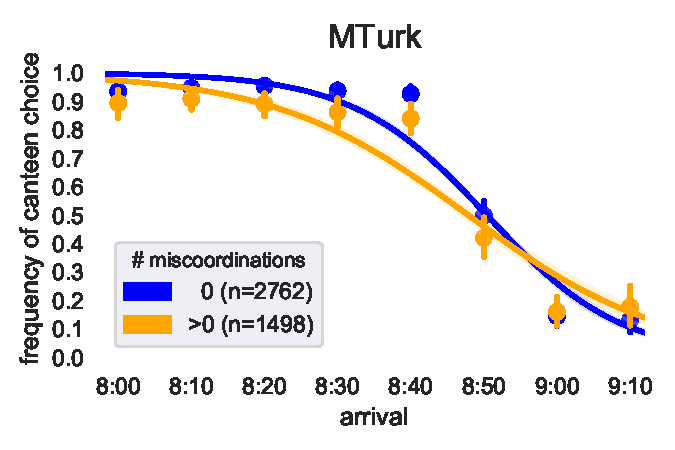
\includegraphics[width=.46\linewidth]{figS6_logit_2bins_MTurk}%
}\hfill
\subfloat[\label{fig: logit dtu}]{%
  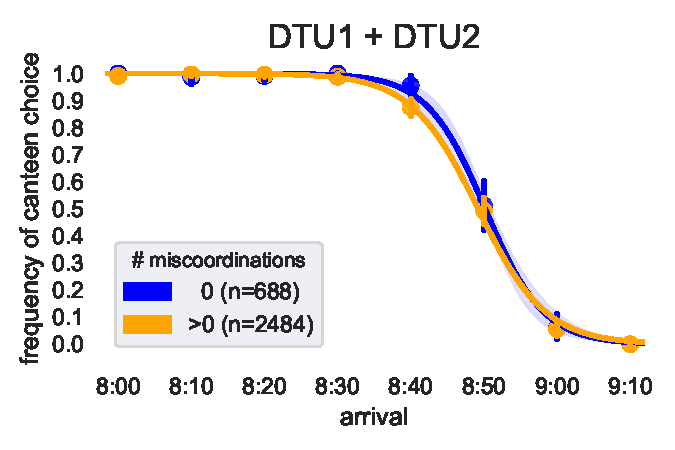
\includegraphics[width=.46\linewidth]{figS6_logit_2bins_DTU}%
}\hfill
\caption{Participant's decisions of going to the canteen as a function of their arrival time, here partitioned into those groups who previous have experienced zero (blue) or one or more (orange) miscoordinations. MTurk participants are shown one the left, DTU students on the right}\label{fig:miscoordinations}
\subfloat[\label{fig: certain mturk}]{%
  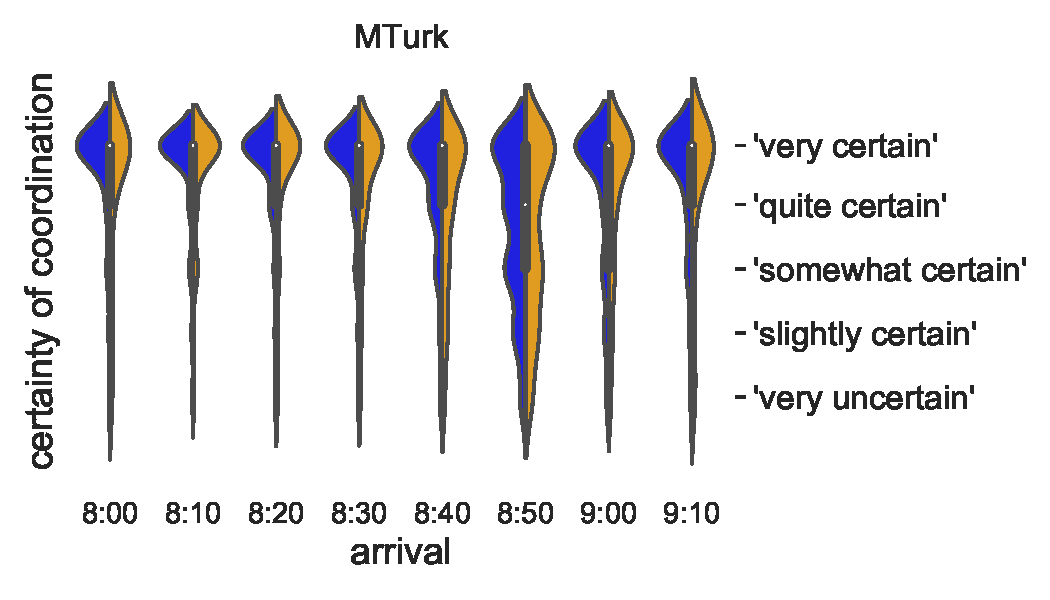
\includegraphics[width=.46\linewidth]{figS7_certainties_MTurk}%
}
\subfloat[\label{fig: certain dtu}]{%
  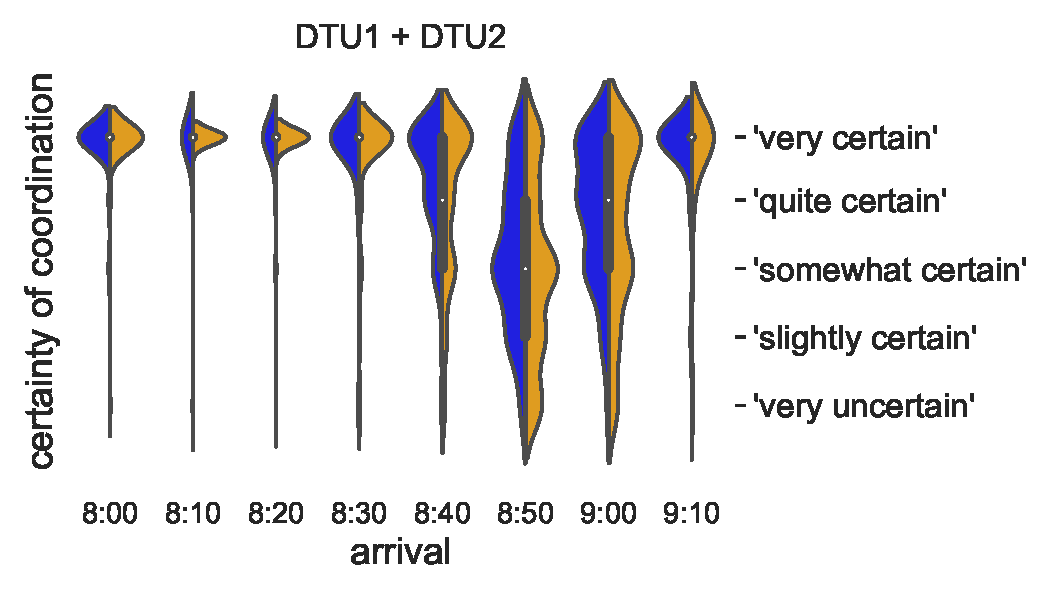
\includegraphics[width=.46\linewidth]{figS7_certainties_DTU}%
}
\caption{Participant's certainty estimates of being able to coordinate with their colleauge as a function of their arrival time, partitioned into those groups who previous have experienced zero (blue) or one or more (orange) miscoordinations. MTurk participants are shown one the left, DTU students on the right}\label{fig:certainties}
\end{figure} 
When a group experiences a round of miscoordination, we expect some kind of learning to take place. `Why did my colleague choose differently than I did?' should be an obvious question a player asks herself, prompting deeper perspective-taking and possibly an understanding of the lack of common knowledge. We investigate this by partitioning decisions into those in which a participant never before has experienced a miscoodination with her colleague ($m=0$) and those in which a participant has experienced one or more miscoodinations ($m>0$). Furthermore, since the number of rounds - and hence miscoordinations - are very different for MTurk participants and DTU students, results from MTurk and DTU are shown separately, with the two DTU experiments combined. Results for the choices in Fig.~\ref{fig:miscoordinations} show significant differences between MTurk-groups having miscoordinated or not, while for DTU students those differences are not significant. Looking into the corresponding certainty estimates, as shown in Fig.~\ref{fig:certainties}, we see a similar pattern as before: Much steeper profiles among DTU students, but also much lower certainty estimates around critical arrival times. 

\iffalse
\section*{Datasets}
MTurk\_anonymous.xlsx, DTU1\_anonymous.xlsx, and DTU2\_anonymous.xlsx: Anonymized data set of all Mechanical Turk experiments. Parameters: session = name of experiment; code = anonymized participant id; group = group number in session; id\_in\_group = player id in group; round = round number; arrival = arrival time; choice = choice made by participant; certainty = certainty estimate by participant; bonus = penalty in dollars; strategy = free text question after game has ended; simple = answers to question 4, cutoff = answers to question 3; fault = answers to question 1; payoff = money left after game has finished.
\fi

\begin{thebibliography}{71}\small
\expandafter\ifx\csname natexlab\endcsname\relax\def\natexlab#1{#1}\fi
\providecommand{\bibinfo}[2]{#2}
\ifx\xfnm\relax \def\xfnm[#1]{\unskip,\space#1}\fi

\bibitem[{Birch and Bloom(2007)}]{birch2007curse}
\bibinfo{author}{S.~A. Birch}, \bibinfo{author}{P.~Bloom},
\newblock \bibinfo{title}{The curse of knowledge in reasoning about false
  beliefs},
\newblock \bibinfo{journal}{Psychological Science} \bibinfo{volume}{18}
  (\bibinfo{year}{2007}) \bibinfo{pages}{382--386}.

\bibitem[{Hara et al. (2018)}]{HaraEtAl18}
\bibinfo{author}{K. Hara}, \bibinfo{author}{et al.},
\newblock \bibinfo{title}{A data-driven analysis of workers' earnings on amazon
  mechanical turk},
\newblock \bibinfo{journal}{Proc. of the 2018 Conference on Human Factors in
  Computing Systems ACM}
  (\bibinfo{year}{2018}) \bibinfo{pages}{449}.

\bibitem[{Zhou and Fishbach(2016)}]{ZhouFishbach16}
\bibinfo{author}{H. Zhou}, \bibinfo{author}{A. Fishbach},
\newblock \bibinfo{title}{The pitfall of experimenting on the web: How
  unattended selective attrition leads to surprising (yet false) research
  conclusions},
\newblock \bibinfo{journal}{Journal of Personality and Social Psychology} \bibinfo{volume}{111}
  (\bibinfo{year}{2016}) \bibinfo{pages}{493--504}.

\bibitem[{Rand (2012)}]{Rand2012}
\bibinfo{author}{D. G. Rand}, \bibinfo{author}{P.~Bloom},
\newblock \bibinfo{title}{The promise of {M}echanical {T}urk: how online labor markets can
  help theorists run behavioral experiments},
\newblock \bibinfo{journal}{Journal of Theoretical Biology} \bibinfo{volume}{299}
  (\bibinfo{year}{2012}) \bibinfo{pages}{172--9}.

\bibitem[{Herzig and Maffre (2015)}]{herzig2015share}
\bibinfo{author}{A. Herzig}, \bibinfo{author}{F. Maffre},
\newblock \bibinfo{title}{How to share knowledge by gossiping},
\newblock \bibinfo{journal}{Springer}
  (\bibinfo{year}{2015}) \bibinfo{pages}{249--263}.

\bibitem[{De~Freitas et~al.(2019)De~Freitas, Thomas, DeScioli, and
  Pinker}]{de2019common}
\bibinfo{author}{J.~De~Freitas}, \bibinfo{author}{K. A.~Thomas},
  \bibinfo{author}{P.~DeScioli}, \bibinfo{author}{S.~Pinker},
\newblock \bibinfo{title}{Common knowledge, coordination, and strategic
  mentalizing in human social life},
\newblock \bibinfo{journal}{Proceedings of the National Academy of Sciences}
  \bibinfo{volume}{116} (\bibinfo{year}{2019}) \bibinfo{pages}{13751--13758}.
\end{thebibliography}
\end{document}